
\chapter{DISCUSSÃO DE RESULTADOS} 

	\par Neste capítulo serão discutidos os principais pontos em relação 
aos resultados obtidos com a execução desta pesquisa. Espera-se com isso
elucidar algumas questões referentes ao modo como a aplicação das teorias
descritas no quadro teórico desta, refletiram na prática.

	\par O sistema operacional \textit{Android} mostrou o porquê de ser tão
utilizado nos dias atuais. Com uma gama enorme de recursos totalmente gratuitos
e com a documentação excelente torna-se claro o que cada função realiza, com
decorrer do desenvolvimento do aplicativo.

	\par Como se constatou que os alunos, na maioria das vezes, acessam o portal
do aluno para consultar notas, faltas e provas agendadas, o aplicativo tem
como importância facilitar para que os discentes tenham suas informações de
maneira fácil e rápida. É notório que é mais simples acessar esses dados pelos
\textit{smartphones} do que por \textit{desktops}, dessa maneira, quando um
professor lançar uma determinada nota, o aluno será notificado de que alguma
informação nova está no portal, evitando que tenha que ficar entrando no portal
várias vezes ao dia ansioso em saber sua média final.

	\par O aplicativo é de fácil utilização, pois com a \textit{activity}
principal, do tipo \textit{Navigation Drawer Layout}, faz com que ele fique
mais atraente, uma vez que o menu fica escondido e apenas é visível se chamado
pelo estudante, além de facilitar aos usuário encontrar as opções por ele
desejada, pois as possibilidades de navegação encontram-se em uma lista. A
seguir pode-se ver a Figura \ref{fig:dr1} do menu. Quando o usuário clicar
no ícone em destaque aparecerá as opções de navegação.

\begin{figure}[h!]
	\centerline{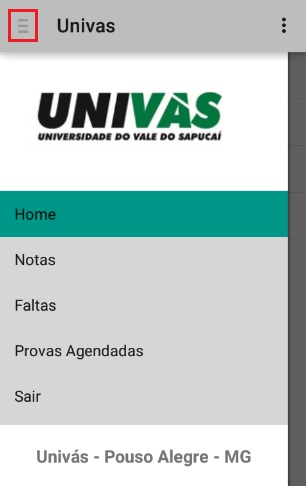
\includegraphics[scale=0.5]{./imagens/3_discussao_resultados/dr1.png}}
	\caption[Menu do Aplicativo]{Menu do Aplicativo.
		\textbf{Fonte:}Elaborado pelos autores.}
	\label{fig:dr1}
\end{figure}
\pagebreak

	\par Quanto a lista de sites que aparecem na \textit{Home}, o resultado não foi
muito empolgante, pois os sites não tornaram-se responsivo, criando barras de
rolagem e gerando desconforto ao usuário conforme mostra a Figura
\ref{fig:dr2}. Contudo há a possibilidade de abrir o site em um navegador,
porém foi analisado e constatado que não seria uma boa prática fazer um usuário
sair do aplicativo.

\begin{figure}[h!]
	\centerline{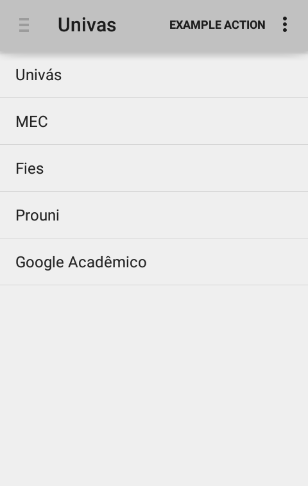
\includegraphics[scale=0.5]{./imagens/3_discussao_resultados/dr2.png}}
	\caption[Navegador Interno Do Aplicativo]{Navegador Interno Do Aplicativo.
		\textbf{Fonte:}Elaborado pelos autores.}
	\label{fig:dr2}
\end{figure}
	
	\par As informações referentes às notas, faltas e provas agendadas estão sendo
apresentadas em uma lista do tipo \textit{ExpadableListView}, este, traz a
vantagem que quando clicado em um de seus itens, é apresentado os seus itens
filhos, por essa razão é desnecessário abrir uma outra \textit{activity},
ficando mais agradável ao usuário e melhorando o desempenho do
\textit{software}. Abaixo, na Figura \ref{fig:dr3} é possível ver a
\textit{activity} de notas, listando algumas informações com \textit{widget
ExpadableListView}.

\begin{figure}[h!]
	\centerline{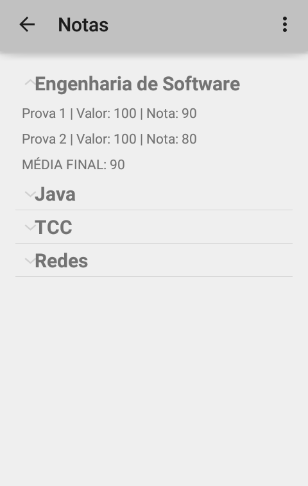
\includegraphics[scale=0.5]{./imagens/3_discussao_resultados/dr3.png}}
	\caption[Tela de Apresentação de notas, faltas e provas agendadas]{Tela de
	Apresentação de notas, faltas e provas agendadas.
		\textbf{Fonte:}Elaborado pelos autores.}
	\label{fig:dr3}
\end{figure}

	\par As informações que vem do \textit{web service} estão sendo salvas no banco
de dados \textit{Sqlite} do aplicativo que mostra-se muito eficiente, uma vez
que é rápido e leve. 

	\par O aplicativo resultado desta pesquisa, tinha necessidade de consumir
dados para posteriormente apresentá-los ao usuário. Era necessário que, os
dados do sistema acadêmico da instituição de ensino que serviu como contexto
para esta pesquisa, fossem transmitidos de alguma forma ao aplicativo. Era
necessário também que os dados chegassem ao aplicativo respeitando as
particularidades de cada usuário, trazendo somente informações relevantes aos
mesmos. Com esse intuito de disponibilizar informações já citadas
anteriormente, a quem quer que fosse necessário, inclusive aos usuários do
aplicativo, foi criado um \textit{Web Service} REST. Este foi um dos resultados
alcançados através desta pesquisa.
	
	\par A construção do \textit{web service}, de ínicio, mostrava-se um tanto
quanto custosa, devido a restrições das tecnologias que foram escolhidas. Por se
tratar de uma simples \textit{web service} que seria disponibilizado para suplir
a demanda de dados do aplicativo, os primeiros serviços foram construídos e
disponibilizados fazendo uso de \textit{servlets} simples e conexão
JDBC\footnote{JDBC - \textit{Java Database Connectivity}}. Este modo como foi
pensado inicialmente, era simples de ser contruído e de uma
\textit{performance} aceitável. 

	\par Porém de acordo com o crescimento da demanda do serviço, tornou-se
inviável a contrução do mesmo com estas técnologias, devido a complexidade com
que era necessário contruir os serviços, haja vista que, com estas técnologias
era necessário que se fosse configurado praticamente tudo de forma manual
inclusive tratamento de erros da aplicação, respostas as requisições e tipos de
dados. Esta etapa teve, portanto, um resultado não muito amigável do ponto de
vista de sua construção. No entanto se for analizado do ponto de vista do
conhecimento adquirido, obteve-se um resulatdo satisfatório, pois, foi na
pesquisa e na busca melhores alternativas a estas técnologias, que se chegou ao
resultado final.

	\par O \textit{web service} foi desenvolvido com algumas técnolgias que
facilitaram a sua construção. Foi usado o \textit{framework Jersey} para prover
os serviços necessários. Este \textit{framework} usa \textit{servlets} para
disponibilizar os serviços, porém com a facilidade de já ter embutido em si o
tratamento para qualquer um dos tipos de dados que usado na implementação de um
serviço REST, tanto para entrada ou saida de dados. Foi ainda usado o
\textit{framework} de pesistência de dados \textit{Hibernate}. Este por sua vez
desenpenhou papel notório, pois, ao mesmo tempo que facilitou o desenvolvimento
do \textit{web service} com relação ao foco nas regras de negócio da aplicação e
não tanto na implementação, pode-se dizer que se, por algum motivo for
necessário migrar de banco de dados este será um fator facilitador. O resultado
final foi extremamente satisfatório, pois era notório que era facíl tanto
contruir e disponibilizar um novo serviço, quanto consumir o mesmo.

	
	\par Para que houvesse dados para que o \textit{web service} transmitisse para
o aplicativo, era necessário receber os dados do sistema acadêmico da referida
instituição, haja vista que o \textit{web service} é independente do sistema
acadêmico desta instituição. Para esse propósito foi construído um módulo que
era responsável por fazer a importação dos dados necessários para a base de
dados do \textit{web service}. Este por sua vez tinha a responsabilidade de
fazer a importação dos dados periodicamente, e ainda tratar os tipos de dados
recebidos para tipos aplicáveis ao banco de dados local. Além disso era
preciso notificar o módulo responsável por invocar o serviço \textit{Google
Cloud Messaging} para que os dispositivos dos alunos aos quais houveram
atualizações nos dados, fossem notificados e fizessem acesso ao \textit{web
service} para solicitar esses dados atualizados. Pode-se dizer então, que este
módulo desempenhou perfeitamente seu papel, pois, com ele era facil manter os
discentes atualizados em relação aos seus dados e ao banco de dados do
\textit{web service} também atualizado e com uma estrutura que fosse condizente
com seus propósitos preestabelecido. 
	
	\par Portanto, conclui-se que se for analizado estes resultados citados de
forma conjunta, pode-se dizer que o resultado geral foi satisfatório, pois, os
discentes puderam obter as informações de que mais fazem uso de forma prática e
rápida.


